%% Author_tex.tex
%% V1.0
%% 2012/13/12
%% developed by Techset
%%
%% This file describes the coding for rsproca.cls

\documentclass{rsproca}%%%%where rsproca is the template name

\RequirePackage{fix-cm}
\usepackage{caption}
\usepackage{subcaption}

%%%% *** Do not adjust lengths that control margins, column widths, etc. ***

%%%%%%%%%%% Defining Enunciations  %%%%%%%%%%%
\newtheorem{theorem}{\bf Theorem}[section]
\newtheorem{condition}{\bf Condition}[section]
\newtheorem{corollary}{\bf Corollary}[section]
%%%%%%%%%%%%%%%%%%%%%%%%%%%%%%%%%%%%%%%%%%%%%%%

\jname{rspa}
\Journal{Proc R Soc A\ }

\begin{document}

%%%% Article title to be placed here
\title{Numerical Solutions of Semi-classical Ellipsoidal-Statistical Bhatnagar-Gross-Krook Model Boltzmann Equation for Two-Dimensional Riemann Problems}

\author{%%%% Author details
Jaw-Yen Yang$^{1,2}$, Zhi-Yuan Yen$^{1}$, Manuel Diaz$^{1}$, Juan-Chen Huang$^{3}$, Zhi-Hui Li$^{4}$}

%%%%%%%%% Insert author address here
\address{$^{1}$Institute of Applied Mechanics, National Taiwan University, Taipei 10764, TAIWAN\\
$^{2}$Center of Quantum Science and Engineering, National Taiwan University, Taipei 10764, TAIWAN\\
$^{3}$Department of Merchant, National Taiwan Ocean University, Taipei 10764, TAIWAN\\
$^{4}$China Aerodynamics Research and Development Center, Mianyang, 10764, CHINA}


%%%% Subject entries to be placed here %%%%
\subject{Mesoscopic Methods, Semi-classical Botlzmann Transport, Ellipsoidal Statistics, Kinetic Theory, Quantum shock waves}

%%%% Keyword entries to be placed here %%%%
\keywords{Semi-classical Boltzmann-ES Equation, Weighted Essentially Non-Oscillatory Scheme, Discrete Ordinate Method, Ellipsoidal Statistical Bhatnagar-Gross-Krook, Two-dimensional Riemann Problems}

%%%% Insert corresponding author and its email address}
\corres{Jaw-Yen Yang\\
\email{yangjy@spring.iam.ntu.edu.tw}}

%%%% Abstract text to be placed here %%%%%%%%%%%%
\begin{abstract}
The ideal quantum gas dynamics as manifested by the semiclassical ellipsoidal statistical equilibrium distribution function as derived in \cite{Wu2012} is computationally studied for particles of three statistics.  This anisotropic ellipsoidal statistical equilibrium distribution was derived through maximum entropy principle and conserves the mass, momentum and energy but differs from the standard Fermi-Dirac or Bose-Einstein distribution. The present numerical method combines the discrete velocity (or momentum) ordinate method in momentum space and high resolution shock capturing method in physical space.   A decoding procedure to obtain the necessary parameters for determining the ellipsoidal equilibrium distribution function is also devised.  Computations of two-dimensional Riemann problems are presented and the results depict the main flow features of the complex nonlinear wave interaction and their manifestation.
\end{abstract}
%%%%%%%%%%%%%%%%%%%%%%%%%%%

%%%%%%%%%% Insert the texts which can accomdate on firstpage in the tag "fmtext" %%%%%

%\begin{fmtext}
%\section{Introduction}
%This is just an example
%\end{fmtext}

%%%%%%%%%%%%%%% End of first page %%%%%%%%%%%%%%%%%%%%%

\maketitle

\section{Introduction}
\label{sec:1}

 The Boltzmann equation has been widely used in kinetic theory of gases to describe various transport phenomena in classical dilute gas covering wide range of flow parameters such as Reynolds number, Mach number and Knudsen number.   The Chapman-Enskog expansion method is usually applied to the Boltzmann equation to derive closed sets of hydrodynamic transport equations, such as Euler and Navier-Stokes equations and beyond that apply to a broad range of flow regimes, see \cite{Cowling1970}.  Analogous to the classical Boltzmann equation, a semiclassical Boltzmann equation, which generalizing the collision term to treat collision of particles of quantum statistics, has been developed \cite{PhysRev.43.552}, see \cite{KadanoffBaym,PhysRev.43.552}.   Hydrodynamic behaviour of quantum gases has been the subject of some prominent researches, see \cite{nikuni98,PhysRev.40.749,PhysRevB.35.7959}, and the application of quantum Boltzmann hydrodynamic equations have been implemented in the analysis of electron flows in quantum semiconductor devices, see \cite{Gardner1994,PhysRevB.39.9536,Woolard5146296}.
In recent years, due to the rapid advancements of nanotechnology, the device or structure characteristic length scales become comparable to the mean free path and the wavelength of energy and information carriers (mainly electrons, photons, phonons, and molecules), some of the classical continuum transport laws are no longer applicable.   It is generally believed that the microscopic description of Boltzmann equation (classical and semiclassical) is adequate to treat transport phenomena in the mesoscale range.  Besides, due to the different types of carriers may involve simultaneously in a single problem, it is desirable to have a method that can allow one to treat them in a unified and parallel manner.   Indeed, this is the view advocated in micro- and nano-scale energy transport by Chen \cite{mit2005nanoscale}.   With the semiclassical Boltzmann equation, it is possible to describe adequately the mesoscale transport of particles of arbitrary statistics.

The principal difficulty encountered in solving semiclassical Boltzmann equation as derived by Uehling and Uhlenbeck is the similar to that encountered in the classical counterpart and is mainly due to the complicated integral nature of its collision term. The relaxation time approximation proposed by Bhatnagar, Gross and Krook (BGK) \cite{PhysRev.94.511} for the classical Boltzmann equation provides a simple form of collision term and retains the principal effects of particle collisions and enables more tractable solution methods.  The relaxation time concept is quite general and is applicable to the semiclassical Boltzmann equation.   The only change is that the equilibrium Maxwell-Boltzmann distribution in the classical case is replaced by the Bose-Einstein or Fermi-Dirac distribution depending on the types of carrier particles.  Indeed, the semiclassical Boltzmann-BGK equation has been widely used in electron carrier transport in semiconductor \cite{Lundstrom:2000,Fatemi1993209,Carrillo2003498,Majorana2001649,Carrillo2003JCEL,Carrillo2003b,Markowich2002,Pattamatta2009,Scaldaferri2007} and phonon energy transport in thermoelectric materials \cite{mit2005nanoscale}.   The main shortcoming of the classical BGK model is that the Prandtl number is equal to one while it is $2/3$ from the full Boltzmann equation.  In order to improve the semiclassical Boltzmann-BGK model equation which does not produce correct Prandtl numbers, a new kinetic model for quantum gases in the normal phase has been developed by Wu, Meng and Zhang \cite{Wu2012}. This new model mimics the classical ellipsoidal statistical (ES) model of Holway \cite{Holway1658} and was derived by maximizing the corresponding entropy function under some constraints.   It posseses all the desirable features of a kinetic model and yields a correct Prandtl number for Fermi gases.   The main purpose of the present work to develop direct solver in phase space for the semiclassical ellipsoidal statistical Boltzmann model equation and calculate rarefied gas flows of arbitrary statistics governing by the semiclassical ES Boltzmann model equation.

In this work, we aim at developing an accurate direct solver for the semiclassical Boltzmann-ES equation in phase space that can treat particles of three statistics on equal foot and in a parallel manner.   Such a method will allow one to examine the same physical flow problems but with different gas of particles.   Also, if the classical limit situations of the same flow problem are considered, then one expect to obtain similar or identical flow structures for the three statistics.   It is noted that even with the classical Maxwell-Boltzmann statistics, the present formulation includes the fugacity which is not seen in the original Boltzmann-BGK equation \cite{PhysRev.94.511} and most other existing works based on it.   First, depending on the carrier particles, the discrete ordinate method is used to discretize the velocity (or momentum or wave number) space in the semiclassical Boltzmann-BGK equation into a set of equations for the discrete distribution functions which are continuous in physical space with source terms \cite{Yang1995323}.  Second, the resulting equations can be treated as scalar hyperbolic conservation law with stiff source term whose evolution in space and time can be modeled by existing shock-capturing schemes such as total variation diminishing (TVD) schemes \cite{Harten1983357} and weighted essentially non-oscillatory (WENO) schemes \cite{Xu2005458}.  The latter is adopted in this paper to describe the evolution of these equations.   We develop the method in two space dimensions and validate the method using flow problems of one and two space dimensions.  Three main aspects of the developed method are examined and emphasized, namely, the range of relaxation time, the range of Knudsen numbers and the recovery of the classical limit.  After the success of these tests, the present method can provide a viable robust tool for treating many modern mesoscale carrier transport phenomena covering electrons and phonons in addition to the usual classical gas molecules.
In the area of classical gas flows, the implementation of discrete ordinate method to nonlinear model Boltzmann equations has been developed by Yang and Huang \cite{Yang1995323} for the rarefied flow computations and has been able to cover broad range of flow regimes.  A WENO-solver
for the 1-D non-stationary electron Boltzmann-Poisson system for semiconductor devices has been presented \cite{Carrillo2003498}. Under the same motivation, this present work is built using discrete ordinate method to describe the hydrodynamic properties of rarefied gases of all the three statistics.

%%E. Fatemi and F. Odeh, Upwind finite difference solution of Boltzmann equation
%%applied to electron transport in semiconductor devices, J. Comput. Phys., 108(1993),
%%209-217.

%%A. Majorana and R. M. Pidatella, A finite difference scheme solving the Boltzmann-
%%Poisson system for semiconductor devices, J. Comput. Phys., 174(2001), 649-668.

%J. A. Carrillo, I. M. Gamba, A. Majorana and C.-W. Shu, A WENO-solver for 1D
%non-stationary Boltzmann-Poisson system for semiconductor devices, J. Comp. Electr.,
%1(2002), 365-375.


%%J. A. Carrillo, I. M. Gamba, A. Majorana and C.-W. Shu, A WENO-solver for
%%the transients of Boltzmann-Poisson system for semiconductor devices. Performance and
%%comparisons with Monte Carlo methods, J. Comp. Phys., 184(2003), 498-525.

%J. A. Carrillo, I. M. Gamba, A. Majorana and C.-W. Shu, A direct solver for
%2D non-stationary Boltzmann-Poisson systems for semiconductor devices: a MESFET
%simulation by WENO-Boltzmann schemes, J. Comput. Electr. 2(2003), 375-380.

%P. A. Markowich, C. Ringhofer and C. Schmeiser, Semiconductor Equations, Springer-
%Verlag, New York, 1990.

%S. Scaldaferri, G. Curatola, and G. Iannaccone,
%Direct Solution of the Boltzmann Transport Equation and Poisson Schrodinger Equation
%for Nanoscale MOSFETs, IEEE TRANSACTIONS ON ELECTRON DEVICES, VOL. 54, NO. 11, NOVEMBER 2007 2901.

%A. Pattamatta and C. K. Madnia, Modeling Electron-Phonon Nonequilibrium in Gold Films
%Using Boltzmann Transport Model, Journal of Heat Transfer,ASME AUGUST 2009, Vol. 131 / 082401-1

% L. Wu, J. Meng and Y. Zhang, Kinetic modelling of the quantum gases in the normal phase, Proc. R. Soc. A, 2012, doi: 10.1098/rspa.2011.0673.

Elements of semiclassical Boltzmann-ES equation is briefly described in Section \ref{sec:2}. Its correlation with hydrodynamic equations is outlined. In Section \ref{sec:3}, we describe the use of discrete ordinate method to discretize the particle distribution function into a set of hyperbolic conservation laws with source terms. In the next section, we present the description of fifth-order WENO scheme implementation in capturing the evolution of discretized distribution function equations. In Section \ref{results}, numerical experiments of one dimensional semiclassical gas dynamical flows in a shock tube in addition to two dimensional Riemann problems are presented to illustrate the present algorithm. Finally, concluding remarks will be given in Section \ref{remarks}.

\section{Semiclassical Ellipsoidal Statistical Boltzmann Model Equation}
\label{sec:2}
In this section, the elements of semiclassical ellipsoidal statistical model Boltzmann equation are briefly described.   Following \cite{PhysRev.43.552,KadanoffBaym}, we consider the extension of the Boltzmann equation to quantum systems due to Uehling and Uhlenbeck  in which they took the Pauli exclusion principle into account.
%%
\begin{equation}
\left(\frac{\partial f}{\partial t}+\frac{\bf p}{m}\cdot {\bf\nabla }_x-{\bf \nabla}_{\bf x} U({\bf x},t)\cdot {\bf\nabla }_{\bf p}\right)f\left({\bf p},{\bf x},t\right)=\left(\frac{\delta f}{\delta t}\right)^{UU}_{coll.}
\end{equation}
where $m$ is the particle mass, $U$ is the mean field potential and $f(\vec p, \vec x, t)$ is the distribution function
which represents the average density of particles with momentum $\vec p$ at the space-time point $\vec x, t$. The $(\delta f
/\delta t)_{coll.}$ denotes the collision term and according to Uehling and Uhlenbeck \cite{PhysRev.43.552}, it takes the form,
\begin{align}
(\frac{\delta f} {\delta t})^{UU}_{coll.} &= \int d {\bf p} \int d\Omega
K({\bf p}, {\bf q}, \Omega) \{ [ 1+ \theta f({\bf p}, t)][1+ \theta f({\bf q})]f({\bf p}^*, t)f({\bf q}^*, t) \nonumber \\
&- [ 1+ \theta f({\bf p}^*, t)][1+ \theta f({\bf q}^*)]f({\bf p}, t)f({\bf q}, t) \},
\end{align}
where $K({\bf p}, {\bf q}, \Omega)$ denotes the collision kernel and $\Omega$ is the solid angle and $\theta$ is a parameter which specifies the type of particle statistics.   Here, for $\theta=+1$, Bose-Einstein particles are considered, for $\theta=-1$, Fermi-Dirac particles, and for $\theta=0$, the Maxwell-Boltzmann classical particles are considered.  It is well known that the collision integral of the semiclassical Boltzmann equation will automatically vanish when the distribution functions are in equilibrium and the equilibrium distribution function for general statistics can be expressed as
\begin{equation}
f^{eq}\left({\bf p},{\bf x},t\right) =\frac{1}{z^{-1}\,exp\left\{{\left[{\bf p}-m\,{\bf u}({\bf x},t) \right]}^2/2mk_BT({\bf x},t)\right\} -\theta }
\end{equation}
where $ {\bf u}({\bf x},t)$ is the, mean velocity, $T({\bf x},t)$ is temperature, $k_B$ is the Boltzmann constant and $z\left({\bf x},t\right)= exp\left({\mu ({\bf x},t)/k_BT({\bf x},t)}\right)$ is the fugacity, where $\mu$ is the chemical potential.  In (\ref{eq:3}), \(\theta=-1\), denotes the Fermi-Dirac statistics, \(\theta=+1\), the Bose-Einstein statistics and \(\theta=0\) denotes the Maxwell-Boltzmann statistics.
To avoid the mathematical difficulty caused by the nonlinear integral collision term, the relaxation time approximation of Bhatnagar, Gross and Krook (BGK) is generally applied to replace the collision term of Uehling and Uhlenbeck, thus the semiclassical Boltzmann-BGK equation reads
\begin{equation}
\left(\frac{\partial f}{\partial t}+\frac{\bf p}{m}\cdot {\bf\nabla }_x-{\bf \nabla}_{\bf x} U({\bf x},t)\cdot {\bf\nabla }_{\bf p}\right)f\left({\bf p},{\bf x},t\right) =\left(\frac{\delta f}{\delta t}\right)_{coll.}= -\ \frac{f-f^{eq}}{\tau }
\end{equation}
where $\tau$ is the relaxation time and and needs to be specified for each carrier scattering.
Using the maximum entropy principle, a new kinetic model equation has been proposed for dilute quantum gases in the normal phase \cite{Holway1658}.  This kinetic model equation preserves the main properties of the semiclassical Boltzmann equation, including conservation of mass, momentum and energy, the entropy dissipation property and the rotational invariance.   It also can provide correct Prandtl numbers.   This semiclaasical ellipsoidal-statistical BGK-Boltzmann equation can be expressed as
\begin{equation}
\left(\frac{\partial f}{\partial t}+\frac{\bf p}{m}\cdot {\bf\nabla }_x-{\bf \nabla}_{\bf x} U({\bf x},t)\cdot {\bf\nabla }_{\bf p}\right)f\left({\bf p},{\bf x},t\right) = -\ \frac{f-f^{ES}}{\tau }
\end{equation}
where $f^{ES}$ is an anisotropic reference equilibrium distribution function given by
\begin{equation}
f^{ES}\left({\bf p},{\bf x},t\right) =\frac{1}{z^{-1}\,exp\left\{{\left[ {1\over 2} \lambda_{\alpha \beta}^{-1} C_{\alpha} C_{\beta} \right]} \right\} -\theta } 
\end{equation}
In Eq. (6), $\lambda_{\alpha \beta}$ is a matrix and $\lambda_{\alpha \beta}^{-1}$ is its inverse and $C_{\alpha} = {p_{\alpha} \over m - u_{\alpha}}$ are the components of the thermal velocity.
It is noted that in Eq. (4), when $f^{ES}$ reduces to $f^{eq}$, Eq. (3), it returns to the BGK model equation.
The reference distribution function is derived by the maximum entropy principle under some constraints that the mass, momentum and energy are conserved and the following relations are satisfied,
\begin{subequations}
\begin{align}
n\left({\bf x},t\right) &= \int{\frac{\ d{\bf p}}{h^D}}\,f_{ES} \left({\bf p},{\bf x}, t\right), \\
\vec u \left({\bf x},t\right) &= \frac{1}{n(\bf x, t)}\int{\frac{\ d{\bf p}}{h^D}\,\frac{\bf p}{m}}\,f_{ES}\left({\bf p},{\bf x}, t\right), \\
P_{\alpha \alpha} \left({\bf x},t\right) &= \int{\frac{\ d{\bf p}}{h^D}\, m C_{\alpha} C_{\alpha} \,f_{ES}\left({\bf p},{\bf x}, t\right)}, \\
W_{\alpha \beta} \left({\bf x},t\right) &= \int{\frac{\ d{\bf p}}{h^D}\,m C_{\alpha} C_{\beta} \,f_{ES} \left({\bf p},{\bf x}, t\right)} 
\end{align}
\end{subequations}
where $D$ is the dimension of momentum space and $W_{\alpha \alpha} = P_{\alpha \alpha}$ is required for the conservation of energy.

The macroscopic dynamic variables of interest such as number density, momentum density and energy density are low order moments of of the distribution function and are defined by:
\begin{subequations}
\begin{align}
n\left({\bf x},t\right) &= \int{\frac{\ d{\bf p}}{h^D}}\,f\left({\bf p},{\bf x}, t\right), \\
\vec u \left({\bf x},t\right) &= {1\over n(\bf x, t) }\int{\frac{\ d{\bf p}}{h^D}\,\frac{\bf p}{m}}\,f\left({\bf p},{\bf x}, t\right), \\
{\epsilon}\left({\bf x},t\right) &= \int{\frac{\ d{\bf p}}{h^D}\,\frac{{\bf p}^2}{2m}}\,f\left({\bf p},{\bf x}, t\right).
\end{align}
\end{subequations}
Other higher-order moments such as pressure tensor $P_{ij}$ and the heat flux vector $Q_i({\bf x},t)$ can also be defined accordingly as
\begin{align}
P_{ij}({\bf x},t) &= \int{\frac{d{\bf p}}{h^D}(\frac{p_i}{m}-u_i)(\frac{p_j}{m}-u_j)\,f\,({\bf p},{\bf x},t)}, \\
Q_i({\bf x},t) &= \int{\frac{d{\bf p}}{h^D}\frac{({\bf p}-m{\bf u})^2}{2m}(\frac{p_i}{m}-u_i)\,f\,({\bf p},{\bf x},t)}.
\label{stressflux}
\end{align}
To determine the reference distribution function or semiclassical ellipsoidal statistical distribution $f^{ES}$, one usually needs to calculate $z$ and the matrix $\lambda_{\alpha \beta}$ simultaneously through
\begin{align}
&({m \over  h})^D \sqrt{ ||2 \pi \lambda_{\alpha \beta}|| } \mathcal{Q}_{D/2}(z)= {\rho \over m}, \\
&({m \over  h})^D \sqrt{ ||2 \pi \lambda_{\alpha \beta}|| } \mathcal{Q}_{D/2 +1}(z) \lambda_{\alpha \beta} = {W_{\alpha \beta} \over m} .
\end{align}
where $||\cdot ||$ denotes the determinant of a matrix.   To determine $W_{\alpha \beta}$ to completely obtain the reference distribution function, a natural choice leading to rotational invariance of the kinetic model equation is (Holway 1966)
\begin{equation}
W_{\alpha \beta}({\bf x},t) = (1 - b) p \delta_{\alpha \beta} + b P_{\alpha \beta}.
\end{equation}
where $p$ is the hydrodynamic pressure defined as the average of the diagonal components of the pressure tensor $P_{\alpha \beta}$, i.e., $p = P_{\alpha \beta}/D$, and $b$ is a parameter.  Requiring $ W_{\alpha \beta}$ to be positive definite, the parameter $b$ satisfies
\begin{align}
-{ 1\over D-1} \le b < 1
\end{align}
for $D=2$ and $D=3$.

The conservation laws of macroscopic properties can be obtained by multiplying Eq. (\ref{eq:1}) respectively by 1, ${\bf p}$ and \({\bf p}^2/2m\)\, and integrating the resulting equations over all ${\bf p}$.  Consequently, the integrals of the collision terms in all three cases vanish automatically resulting in the conservation laws in differential equations form for the conserved macroscopic quantities i.e., number density \(n({\bf x},t)\), momentum density \(m n {\bf u}({\bf x},t)\), and energy density \(\epsilon({\bf x},t)\) as follow:

\begin{align}
\frac{\partial n\left({\bf x},t\right)}{\partial t}&+{\bf \nabla }_x\cdot{\bf j}\left({\bf x},t\right)=0, \\
\frac{\partial m\/{\bf j}\left({\bf x},t\right)}{\partial t}&+{\bf \nabla }_x\cdot\int{\frac{d{\bf p}}{h^3}}\,{\bf p}\,\frac{\bf p}{m}f\left({\bf p},{\bf x},t\right)= -n({\bf x},t){\bf \nabla}_{\bf x}U({\bf x},t), \\
\frac{\partial \epsilon \left({\bf x},t\right)}{\partial t}&+{\bf \nabla }_x\cdot\int{\frac{d\bf p}{h^3}}\,\frac{\bf p}{m}\,\frac{{\bf p}^2}{2m}f\left({\bf p},{\bf x},t\right)=-{\bf j}({\bf x},t)\cdot{\bf \nabla}_{\bf x}U({\bf x},t).
\end{align}

In this work, we will also consider the case of {\em semiclassical Euler} limit in which the particle distribution function is always in reference equilibrium, i.e., $f=f^{ES}$ and the collision term of Eq. (\ref{eq:5}) vanishes automatically.  Following the classical ellipsoidal statistical model, we shall denote the reference distribution function as the semiclassical ES distribution from here on.  In the later section, we will present the comparison of our results with those of the semiclassical Euler solutions.  In recent years, notable numerical methods to describe the ideal quantum gas flows have been developed, see \cite{1272832,Shi20089389,Jaw-YenYang05082006}.

\section{Governing Equations in Two Space Dimensions}
\label{sec:3 1}
We shall give detailed description of the theory and solution method in two space dimensions.   The general method in three space dimensions can be similarly
formulated.   The semiclassical Boltzmann-ES model equation in two space dimensions with $f=f^{ES}$ can be given by
%%
\begin{align}
\frac{\partial f^{ES}({\upsilon}_x,{\upsilon}_y, x, y, t)}{\partial t} + {\upsilon}_x\,\frac{\partial f^{ES}({\upsilon}_x,{\upsilon}_y, x, y, t)}{\partial x } + {\upsilon}_y\,\frac{\partial f^{ES}({\upsilon}_x,{\upsilon}_y, x, y, t)} {\partial y} =0, \label{normalizedes}
\end{align}
%%
with ${\upsilon}_x$ and ${\upsilon}_y$ as particle velocities.   The macroscopic properties are the various moments of $f^{ES}({\upsilon}_x,{\upsilon}_y,x,y,t)$,
\begin{subequations} 
\begin{align}
\rho (x,y,t) 			&= \int \frac{ d p_x}{h} \frac{ d p_y}{h} \, f^{ES}(p_x, p_y, x, y, t), \\
u_x (x,y,t) 			&= \frac{1}{\rho} \int 	 \frac{ d p_x}{h} \, \frac{ d p_y}{h}  p_x \, f^{ES}(p_x, p_y, x, y, t), \\
u_y (x,y,t) 			&= \frac{1}{\rho} \int 	 \frac{ d p_x}{h} \, \frac{ d p_y}{h}  p_y \, f^{ES}(p_x, p_y, x, y, t), \\
\epsilon (x,y,t) 	&= \int \frac{ d p_x}{h} \frac{ d p_y}{h} \, \frac{(p_x^2 + p_y^2)}{2m} \, f^{ES}(p_x, p_y, x, y, t).
\end{align}
\end{subequations}
Additional information from $f^{ES}$ can also be defined accordingly to
\begin{subequations}
\begin{align}
W_{x x}(x,y,t)	&=	\int \frac{ d p_x}{h} \frac{ d p_y}{h} \, (\frac{p_x}{m}-u_x)(\frac{p_x}{m}-u_x)\,f^{ES}(p_x, p_y, x, y, t), \\
W_{x y}(x,y,t)	&=	\int \frac{ d p_x}{h} \frac{ d p_y}{h} \, (\frac{p_x}{m}-u_x)(\frac{p_y}{m}-u_y)\,f^{ES}(p_x, p_y, x, y, t), \\
W_{y y}(x,y,t)	&=	\int \frac{ d p_x}{h} \frac{ d p_y}{h} \, (\frac{p_y}{m}-u_y)(\frac{p_y}{m}-u_y)\,f^{ES}(p_x, p_y, x, y, t). 
\end{align}
\end{subequations}
We also have the gas pressure $p(x,y,t) = {W_{xx} + W_{yy} \over 2}$.  The pressure tensor $P_{\alpha \beta}(x,y,t)$ can be obtained through
\begin{equation}
P_{xx} = [W_{xx} - (1-b)p]/b, \,\, P_{xy} = W_{xx}/b, \,\, P_{yy} = [W_{yy} - (1-b)p]/b.
\end{equation}
For the conservation of energy, $W_{xx} +W_{yy} = P_{xx} + P_{yy}$ is required.
To obtain the new $f^{ES}$, one needs $z$ and $\lambda_{xx}, \lambda_{xy}\lambda_{yy}$ and these can be determined through solving the following equations simultaneously,
\begin{align}
&({m \over h})^2 \sqrt{||2 \pi \lambda_{\alpha \beta} ||}\mathcal{Q}_{1}(z) = {\rho \over } \nonumber\\
&({m \over h})^2 \sqrt{||2 \pi \lambda_{\alpha \beta} ||}\mathcal{Q}_{2}(z) \lambda_{\alpha \beta}= {W_{\alpha \beta} \over m}.
\end{align}
Computationally, this requires a root finding procedure and either Newton-Ralphson method or bisector method can be employed.

\subsection{Governing Equations in Non-Dimensional Form}
\label{subsec:3_2}
Before proceeding to discretize the equation, in this section we introduce the characteristic properties of $V_0$, $t_0$ and $n_0$ (or $z_0$ ) for the purpose of normalization.  Choose some reference parameters as
\begin{equation}
V_0 = \sqrt{\frac{2k_B T_0}{m}}, \, t_0 = \frac{L}{V_0},\, n_{0} = \frac{2 \pi m k_B T_0}{h^2} \mathcal{Q}_1 (z_0), f_0=\pi \mathcal{Q}_1(z_0).
\end{equation}
%%
with $L$ defined as the characteristic length of the problem. Hence the definitions of non-dimensional variables are introduced as
%%
\begin{align}
\hat{t} &=\frac{t}{t_0},& (\hat{u}_y,\hat{\upsilon_y})&={(u_y,\upsilon_y)\over V_0},& 
(\hat{u}_x,\hat{\upsilon_x})&=\frac{(u_x,\upsilon_x)}{V_0},& (\hat{x},\hat{y})&=\frac{v(x, y)}{L},& \nonumber \\
\hat{T}&=\frac{T}{T_0},& \hat{n}&={n \over \left(\frac{m^2V_0^2}{h^2}\right)}& 
\hat{j}&={j \over \left(\frac{m^2V_{0}^3}{h^2}\right) },& \hat{\epsilon}&={\epsilon \over \left(\frac{m^3 V_{0}^4}{h^2}\right)},& \nonumber \\
& & & &\hat{P_{\alpha \beta}} &= { P_{\alpha \beta} \over n_{0} V_{0}^2 },& \hat{W_{\alpha \beta}} &= { W_{\alpha \beta} \over n_{0} V_0^2}.&
\end{align}
%%
After non-dimensionalizing the equation, we have the normalized semiclassical Boltzmann-ES equation in two space dimensions as follow.
%%
\begin{equation}
\frac{\partial\hat{f}(\hat{\upsilon}_x,\hat{\upsilon}_y,\hat{x},\hat{y},\hat{t})}{\partial\hat{t}} + \hat{\upsilon}_x\,\frac{\partial\hat{f}(\hat{\upsilon}_x,\hat{\upsilon}_y,\hat{x},\hat{y},\hat{t})}{\partial\hat{x}} + \hat{\upsilon}_y\,\frac{\partial\hat{f}(\hat{\upsilon}_x,\hat{\upsilon}_y,\hat{x},\hat{y},\hat{t})}{\partial\hat{y}} = 0, \label{normalizedes}
\end{equation}
%%
with $\hat{\upsilon}_x$ and $\hat{\upsilon}_y$ as particle velocities. The normalized two-dimensional semiclassical reference distribution function becomes
%%
\begin{equation}
\hat{f}^{ES}\left(\hat{\upsilon}_x,\hat{\upsilon}_y,\hat{x},\hat{y},\hat{t}\right) =
\left[ z^{-1}\,\exp\left\{ \frac{1}{2 \hat{\Omega}} \left[ \hat{\lambda_{yy}} \hat{C}_x^2 - 2 
\hat{\lambda_{xy}} \hat{C}_x \hat{C}_y + \hat{\lambda_{xx}} \hat{C}_y^2 \right] + \theta  \right\} \right]^{-1}
\end{equation}
where $\hat{\Omega} = \hat{\lambda_{xx}} \hat{ \lambda_{yy}} - \hat{\lambda_{xy}}^2$.

%%From this part, our formulations are all considered normalized and we shall omit the 'hat' sign for simplicity.

%% The Appendices part is started with the command \appendix;
%% appendix sections are then done as normal sections
%% \appendix

\subsection{Fermi and Bose functions in relation to hydrodynamics properties}
\label{subsec:2_1}

Before we proceed, without losing generality, we neglect the influence of externally applied field \(U({\bf x},t)\). To illustrate the present method, we formulate the reference equilibrium distribution in the case of $D=2$ as the following.
%%
\begin{align}
f^{eq}(p_x,p_y,x,y,t) &= \nonumber \\
&\frac{1}{z^{-1}\,\exp\left\{ \left[ (p_x-mu_x)^2 + (p_y-mu_y)^2 \right]/\left[2mk_BT(x,y,t)\right]\right\}+\theta}
\end{align}
In a closed form in terms of quantum functions, we replace the distribution function $f$ with $f^{eq}$ which automatically reduces the source term in the BGK Boltzmann equation to zero. The macroscopic moments, i.e., number density \(n(x,y,t)\), momentum \(j(x,y,t)\) and energy density \(\epsilon(x,y,t)\) are given by
%%
\begin {align}
n(x,y,t) &= \int\int{\frac{dp_x\,dp_y}{h^2}f^{eq}(p_x,p_y,x,y,t)}\nonumber \\
&= \frac{\mathcal{Q}_{1}(z)}{\lambda}^2  \\
\nonumber \\
j_x(x,y,t) &= \int\int{\frac{dp_x\,dp_y}{h^2}\frac{p_x}{m}f^{eq}(p_x,p_y,x,y,t)}\nonumber \\
&= n(x,y,t)u_x(x,y,t)  \\
\nonumber \\
j_y(x,y,t) &= \int\int{\frac{dp_x\,dp_y}{h^2}\frac{p_y}{m}f^{eq}(p_x,p_y,x,y,t)}\nonumber \\
&= n(x,y,t)u_y(x,y,t)  \\
\nonumber \\
\epsilon(x,y,t) &= \int\int{\frac{dp_x\,dp_y}{h^2}\frac{{p_x}^2+{p_x}^2}{2m}f^{eq}(p_x,p_y,x,y,t)}\nonumber \\
&= \frac{\mathcal{Q}_{2}(z)}{\beta\lambda^2}+\frac{1}{2}mn({u_x}^2+{u_y}^2)\nonumber \\
&= \frac{P(x,y,t)}{(\gamma - 1)}+\frac{1}{2}mn({u_x}^2+{u_y}^2)
\end{align}
where \(\lambda=\sqrt{\frac{\beta h^2}{2\pi m}}\) is the thermal wavelength and \(\beta=1/k_{B} T(x,t)\).  The functions $\mathcal{Q}_{\nu}(z)$ of order $\nu$ are respectively defined for Fermi-Dirac and Bose-Einstein statistics as
%%
\begin {align}
\mathcal{F}_{\nu}(z)&\equiv \frac{1}{\Gamma(\nu)} \int^{\infty}_{0}{dx\frac{x^{\nu -1}}{z^{-1}e^{x} +1}}\approx\sum^{\infty}_{l=1}\,(-1)^{l-1}\,{\frac{z^l}{l^\nu}}\\
\mathcal{B}_{\nu}(z)&\equiv \frac{1}{\Gamma(\nu)} \int^{\infty}_{0}{dx\frac{x^{\nu-1}}{z^{-1}e^{x}-1}}\approx\sum^{\infty}_{l=1}{\frac{z^l}{l^\nu}}
\end{align}
Here,  \(\mathcal{F}_{\nu}(z)\) applies for Fermi-Dirac integral and \(\mathcal{B}_{\nu}(z)\) for Bose-Einstein's, whereas \(\Gamma(\nu)\) is gamma function. The definition of macroscopic quantities in terms of Fermi or Bose function applies for both cases of quantum distributions. One only needs to replace Fermi function with Bose function or vice versa whilst maintaining the same procedure.

In the later section, we shall see the numerical examples that compare Fermi and Bose gas to the classical limit.

\section{ Discrete Ordinate Method and Quadrature Rules}
\label{sec:3}
In two-dimensional case, we may apply Gauss-Hermite quadrature rule over the interval $[-\infty,\infty]$ for each direction.  The Gauss-Hermite quadrature rule reads,
%%
\begin{equation}
\int^{\infty}_{-\infty}\int^{\infty}_{-\infty}{e^{-{\upsilon_x}^2}e^{-{\upsilon_y}^2}f(\upsilon_x,\upsilon_y)d\upsilon_x\,d\upsilon_y} \approx \sum^{N_1}_{\sigma=-N_1}\sum^{N_2}_{\sigma=-N_2}{W_\sigma\,W_\delta\, f_{\sigma,\delta}}
\end{equation}
or
%%
\begin{eqnarray}
\int^{\infty}_{-\infty}\int^{\infty}_{-\infty}{e^{-{\upsilon_x}^2}e^{-{\upsilon_y}^2}\,[e^{{\upsilon_x}^2}e^{{\upsilon_y}^2}f(\upsilon_x,\upsilon_y) d\upsilon_x\,d\upsilon_y]} \approx \nonumber \\
\nonumber \\
\sum^{N_1}_{\sigma=-N_1}\sum^{N_2}_{\sigma=-N_2}{W_\sigma\,W_\delta\,e^{{\upsilon_\sigma}^2}e^{{\upsilon_\delta}^2}f_{\sigma,\delta}}
\end{eqnarray}
The discrete points $\upsilon_\alpha$ and the corresponding weights $W_\alpha$, with $\alpha=\sigma,\delta$, are tabulated in the table of the Gauss-Hermite quadrature, see \cite{abramowitz+stegun}.
%%
\begin{equation}
W_\alpha = \frac{2^{l-1}l!\sqrt{\pi}}{l^2[H_{l-1}(\upsilon_\alpha)]^2}
\label{weightsgh}
\end{equation}
with $l$ is number of quadrature points and $\upsilon_\alpha$ are the roots of the Hermite polynomial \(H_l(\upsilon)\)

Once the discrete distribution functions $f_{\sigma,\delta}(x,y,t)$ are solved, for every time level we can acquire and update the macroscopic moments in the physical space using a selected quadrature method as described below.
% Macroscopic Moments
\begin{align}
	\begin{split}
% Number Density
\rho(x,y,t) &= \int^{\infty}_{-\infty}{[f^{ES}(\upsilon_x,\upsilon_y,x,y,t)e^{{\upsilon_x}^2}\,e^{{\upsilon_y}^2}]e^{-{\upsilon_x}^2}e^{-{\upsilon_y}^2}d\upsilon_x d\upsilon_y}  \\
&=\sum^{N_1}_{\sigma=-N_1}\sum^{N_2}_{\sigma=-N_2}{W_\sigma\,W_\delta\,e^{{\upsilon_\sigma}^2}e^{{\upsilon_\delta}^2}f^{ES}_{\sigma,\delta}} \\
% x-Velocity
u_x(x,y,t) &= {1 \over \rho} \int^{\infty}_{-\infty}{[\upsilon_x\,f^{ES}(\upsilon_x,\upsilon_y,x,y,t)e^{{\upsilon_x}^2}\,e^{{\upsilon_y}^2}]e^{-{\upsilon_x}^2}e^{-{\upsilon_y}^2}d\upsilon_x d\upsilon_y}  \\
&= {1 \over \rho} \sum^{N_1}_{\sigma=-N_1}\sum^{N_2}_{\sigma=-N_2}{\upsilon_\sigma\,W_\sigma\,W_\delta\,e^{{\upsilon_\sigma}^2} e^{{\upsilon_\delta}^2}f^{ES}_{\sigma,\delta}}  \\
% y-Velocity
u_y(x,y,t) &= {1 \over \rho} \int^{\infty}_{-\infty}{[\upsilon_y\,f{ES}(\upsilon_x,\upsilon_y,x,y,t)e^{{\upsilon_x}^2}\,e^{{\upsilon_y}^2}]e^{-{\upsilon_x}^2}e^{-{\upsilon_y}^2}d\upsilon_x d\upsilon_y}  \\
&= {1 \over \rho} \sum^{N_1}_{\sigma=-N_1}\sum^{N_2}_{\sigma=-N_2}{\upsilon_\delta\,W_\sigma\,W_\delta\,e^{{\upsilon_\sigma}^2} e^{{\upsilon_\delta}^2}f{ES}_{\sigma,\delta}} \\
% Energy Density
\epsilon(x,y,t) &= \int^{\infty}_{-\infty}{[\frac{\upsilon^2_x+\upsilon^2_y}{2}\,f^{ES}(\upsilon_x,\upsilon_y,x,y,t)e^{{\upsilon_x}^2}\,e^{{\upsilon_y}^2}] e^{-{\upsilon_x}^2}e^{-{\upsilon_y}^2}d\upsilon_x d\upsilon_y} \\
&= \sum^{N_1}_{\sigma=-N_1}\sum^{N_2}_{\sigma=-N_2}{(\frac{\upsilon^2_\sigma+\upsilon^2_\delta}{2})W_\sigma\,W_\delta\,e^{{\upsilon_\sigma}^2} e^{{\upsilon_\delta}^2}f^{ES}_{\sigma,\delta}} 
	\end{split}
%\label{macrodom1}
\end{align}
and
\begin{align}
	\begin{split}
% xx-Pressure Tensor component 
W_{xx}(x,y,t) &= \int^{\infty}_{-\infty} (\upsilon_x - u_x)^2 \, f^{ES}(\upsilon_x,\upsilon_y,x,y,t) e^{\upsilon_x^2}\,e^{\upsilon_y^2}] e^{-{\upsilon_x}^2} e^{-{\upsilon_y}^2} d\upsilon_x d\upsilon_y \\
&= \sum^{N_1}_{\sigma=-N_1}\sum^{N_2}_{\sigma=-N_2} (\upsilon_{\upsilon_\sigma} - u_x)^2 {\upsilon^2_\sigma})W_\sigma\,W_\delta\,e^{{\upsilon_\sigma}^2}e^{{\upsilon_\delta}^2}f^{ES}_{\sigma,\delta}  \\
% xy-Pressure Tensor component 
W_{xy}(x,y,t) &= \int^{\infty}_{-\infty} (\upsilon_x - u_x) (\upsilon_y - u_y) \, f^{ES}(\upsilon_x,\upsilon_y,x,y,t) e^{\upsilon_x^2}\,e^{\upsilon_y^2}] e^{-{\upsilon_x}^2} e^{-{\upsilon_y}^2} d\upsilon_x d\upsilon_y \\
&= \sum^{N_1}_{\sigma=-N_1}\sum^{N_2}_{\sigma=-N_2} (\upsilon_{\upsilon_\sigma} - u_x) (\upsilon_{\upsilon_\delta} - u_y) {\upsilon^2_\sigma})W_\sigma\,W_\delta\,e^{{\upsilon_\sigma}^2}e^{{\upsilon_\delta}^2}f^{ES}_{\sigma,\delta}  \\
% yy-Pressure Tensor component 
W_{yy}(x,y,t) &= \int^{\infty}_{-\infty} (\upsilon_x - u_x)^2 \, f^{ES}(\upsilon_x,\upsilon_y,x,y,t) e^{\upsilon_x^2}\,e^{\upsilon_y^2}] e^{-{\upsilon_x}^2} e^{-{\upsilon_y}^2} d\upsilon_x d\upsilon_y \\
&= \sum^{N_1}_{\sigma=-N_1}\sum^{N_2}_{\sigma=-N_2} (\upsilon_{\upsilon_\sigma} - u_y)^2 {\upsilon^2_\sigma})W_\sigma\,W_\delta\,e^{{\upsilon_\sigma}^2}e^{{\upsilon_\delta}^2}f^{ES}_{\sigma,\delta}  \\
	\end{split}
%\label{macrodom_cont}
\end{align}
Once the values of $W_{\alpha \beta}$ have been obtained, the pressure and pressure tensor are given by
\begin{align}
	\begin{split}
p(x,y,t) 	&= (W_{xx} + W_{yy})/2, \\
P_{xx} 		&= [W_{xx} - (1-b)p]/b, \\
P_{yy} 		&= [W_{yy} - (1-b)p]/b, \\
P_{xy} 		&= W_{xx}/b.
	\end{split}
\end{align}
Here, we note that the basic criteria of choosing different quadratures is to guarantee that the macroscopic moments can be accurately computed which requiring the accurate representation of the distribution function with suitable velocity range being covered.   The equally spaced Newton-Cotes formula can also be used if one needs to cover the high energy tail of the distribution function.

\section{Numerical Method}
\label{sec:4}
\subsection{Implementation of High Resolution Shock Capturing Schemes}
\label{WENO}
In this section, we describe the numerical algorithm to solve the set  of Eq. (18).  A class of WENO schemes is implemented to solve the set of conservation laws with source terms.   We firstly discretize the space $x,y$  and time $t$ into a number of cells centered at $i,j$ at time $n$, hence we approximate $f^{ES}_{\sigma,\delta}(x,y,t)$ by ${f^{ES}_{\sigma,\delta}}_{i,j}^{n}$. In terms of numerical fluxes, the evolution from $n^{th}$ time level to $(n+1)^{th}$ time level is expressed by

\begin{align}
	\begin{split}
{f^{ES}_{\sigma,\delta}}_{i,j}^{n+1} &= {f^{ES}_{\sigma,\delta}}_{i,j}^{n}
-\frac{\Delta t}{\Delta x}\left(F_{i+1/2,j}^N-F_{i-1/2,j}^N\right) \\
&-\frac{\Delta t}{\Delta y}\left(G_{i,j+1/2}^N - G_{i,j-1/2}^N\right)
	\end{split}
\end{align}
where the numerical fluxes are defined by
\begin{align}
&F_{i+1/2,j}^N=F_{i+1/2,j}^+ + F_{i+1/2,j}^-& &,& &G_{i,j+1/2}^N=G_{i,j+1/2}^+ + G_{i,j+1/2}^-&
\end{align}
where the split flux vectors are defined by
\begin{align}
&F_{i,j}^{+} = \upsilon_\sigma^+ f^{ES}_{\sigma,\delta;i,j}& &F_{i,j}^{-} = \upsilon_\sigma^-f^{ES}_{\sigma,\delta;i,j}& \nonumber \\
&G_{i,j}^{+} = \upsilon_\delta^+ f^{ES}_{\sigma,\delta;i,j}& &G_{i,j}^{-} = \upsilon_\delta^-f^{ES}_{\sigma,\delta;i,j}& 
\end{align}
Here, $\upsilon_\sigma^{\pm} = (\upsilon_\sigma \pm |\upsilon_\sigma |)/2$ and $\upsilon_\delta^{\pm} = (\upsilon_\delta \pm |\upsilon_\delta |)/2$.
In this work, a fifth-order accurate $(r=3)$ WENO (from now on, this will be denoted as WENO3) scheme is considered for the spatial difference of numerical fluxes.   We shall omit the subscripts $(\sigma,\delta)$ and set $F_{i,j}= f^{ES}_{i,j}$ below to save space.
\begin{align}
	\begin{split}
F_{i+1/2,j}^{+} &= \omega_{0}^{+}\left(\frac{2}{6}F_{i-2,j}^+ -\frac{7}{6}F_{i-1,j}^+ +\frac{11}{6}F_{i,j}^+\right) \\
&+ \omega_{1}^{+}\left(-\frac{1}{6}F_{i-1,j}^+ +\frac{5}{6}F_{i,j}^++\frac{2}{6}F_{i+1,j}^+\right) \\
&+ \omega_{2}^{+}\left(\frac{2}{6}F_{i,j}^+ +\frac{5}{6}F_{i+1,j}^+ +\frac{1}{6}F_{i+2,j}^+\right)
	\end{split}
\end{align}

\begin{align}
&\omega_{k}^{+} = \frac{\alpha_{k}^{+}}{\alpha_{0}^{+}+\alpha_{1}^{+}+\alpha_{2}^{+}}& &k = 0,1,2&
\end{align}

\begin{align}
&\alpha_{0}^{+}=\frac{1}{10(\epsilon+IS_{0}^{+})^2}& 
&\alpha_{1}^{+}=\frac{6}{10(\epsilon+IS_{1}^{+})^2}&
&\alpha_{2}^{+}=\frac{3}{10(\epsilon+IS_{2}^{+})^2}&
\end{align}
\begin{align}
	\begin{split}
IS_{0}^+ &= \frac{13}{12}\left(F_{i-2,j}^+ -2F_{i-1,j}^+ +F_{i,j}^+\right)^2 +\frac{1}{4}\left(F_{i-2,j}^+ -4F_{i-1,j}^+ +3F_{i,j}^+\right)^2\\
IS_{1}^+ &= \frac{13}{12}\left(F_{i-1,j}^+ -2F_{i,j}^+ +F_{i+1,j}^+\right)^2 +\frac{1}{4}\left(F_{i-1,j}^+ -F_{i+1,j}^+\right)^2\\
IS_{2}^+ &= \frac{13}{12}\left(F_{i,j}^+ 	 -2F_{i+1,j}^+ +F_{i+2,j}^+\right)^2 +\frac{1}{4}\left(3F_{i,j}^+ -4F_{i+1,j}^+ +F_{i+2,j}^+\right)^2
	\end{split}
\end{align}

The numerical flux for the negative part is given by
\begin{align}
	\begin{split}
F_{i+1/2,j}^-
&= \omega_{0}^{-}\left(-\frac{1}{6}F_{i-1,j}^-  +\frac{5}{6}F_{i,j}^-   +\frac{2}{6}F_{i+1,j}^-\right) \\
&+ \omega_{1}^{-}\left( \frac{2}{6}F_{i,j}^-    +\frac{5}{6}F_{i+1,j}^- -\frac{1}{6}F_{i+2,j}^-\right) \\
&+ \omega_{2}^{-}\left( \frac{11}{6}F_{i+1,j}^- -\frac{7}{6}F_{i+2,j}^- +\frac{2}{6}F_{i+3,j}^-\right)
	\end{split}
\end{align}

\begin{align}
&\omega_{k}^{-} = \frac{\alpha_{k}^{-}}{\alpha_{0}^{-}+\alpha_{1}^{-}+\alpha_{2}^{-}},&  &k = 0,1,2&
\end{align}

\begin{align}
&\alpha_{0}^{-}=\frac{3}{10(\epsilon+IS_{0}^{-})^2}& 
&\alpha_{1}^{-}=\frac{6}{10(\epsilon+IS_{1}^{-})^2}& 
&\alpha_{2}^{-}=\frac{1}{10(\epsilon+IS_{2}^{-})^2}&
\end{align}

\begin{align}
IS_{0}^- &= \frac{13}{12}\left(F_{i-1,j}^- -2F_{i,j}^- +F_{i+1,j}^-\right)^2 +\frac{1}{4}\left(F_{i-1,j}^- -4F_{i,j}^- +3F_{i+1,j}^-\right)^2\\
IS_{1}^- &= \frac{13}{12}\left(F_{i,j}^- -2F_{i+1,j}^- +F_{i+2,j}^-\right)^2 +\frac{1}{4}\left(F_{i,j}^- -F_{i+2,j}^-\right)^2\\
IS_{2}^- &= \frac{13}{12}\left(F_{i+1,j}^- -2F_{i+2,j}^- +F_{i+3,j}^-\right)^2+\frac{1}{4}\left(3F_{i+1,j}^- -4F_{i+2,j}^- +F_{i+3,j}^-\right)^2
\end{align}
The expression of $G_{i,j+1/2}^+$ and $G_{i,j+1/2}^-$ can be derived in a similar fashion.

\subsection{Application of Total Variation Diminishing (TVD) Scheme}
\label{TVD}
For comparison purpose, we also implement a second-order TVD scheme.  Under the same expression as Eq. (\ref{maincv}), we can also define the numerical fluxes for a TVD scheme given by
\begin{eqnarray}
F_{i+1/2,j}^N &=& \left(F_{i+1/2,j}^++F_{i+1/2,j}^-\right)\nonumber\\
&+&\frac{1}{2}\left[{\mbox{sgn}}(\upsilon_{\sigma})-|\upsilon_{\sigma}|\right]\left[\upsilon_\sigma^+\Delta x \phi({\theta_x}_{i,j})+\upsilon_\sigma^-\Delta x \phi({\theta_x}_{i+1,j})\right]
\end{eqnarray}
with $\phi({\theta_x}_{i,j})$ chosen to be the van Leer limiter \cite{vanLeer1979101} given by
\begin{eqnarray}
\phi({\theta_x}_{i,j})&=&\frac{(|{\theta_x}_{i,j}|+{\theta_x}_{i,j})}{1+|{\theta_x}_{i,j}|}\nonumber\\
{\theta_x}_{i,j}&=&\frac{{f_{\sigma,\delta}}_{i'+1,j}^{n}-{f_{\sigma,\delta}}_{i',j}^{n}}{{f_{\sigma,\delta}}_{i+1,j}^{n}-{f_{\sigma,\delta}}_{i,j}^{n}}\,,\hspace{0.1in} i'=i-{\mbox{sgn}}\left(\upsilon_\sigma\frac{\Delta t}{\Delta x}\right)
\end{eqnarray}
The expression of $G_{i,j+1/2}^N$ can be derived similarly. Additionally, the comparison between the results generated using WENO3 and those using TVD will also be given in the later section.
\subsection{Determination of $z$ and $\lambda_{\alpha \beta}$}
After acquiring the macroscopic moments, we need to update the values of $z$ and $\lambda_{\alpha \beta}$ in order to obtain the $f^{ES}$ distribution function for the next time step.  To solve $z(x,y,t)$, which is the root of equation
\begin{equation}
	\Psi_2(z)=\mathcal{Q}_{2}(z)^2 (\rho/\mathcal{Q}_{1}(z))^{4} - 4 (W_{xx} W_{yy} - W_{xy}^2)
\end{equation}
we can use numerical root finding methods.  After the new value of $z$ is determined, we can immediately find $\lambda_{\alpha \beta}$ before advancing the solution to the next time step.
\begin{align}
&\lambda_{xx} = {W_{xx} \over \rho} {\mathcal{Q}_{1}(z) \over \mathcal{Q}_{2}(z)}&
&\lambda_{xy} = {W_{xy} \over \rho} {\mathcal{Q}_{1}(z) \over \mathcal{Q}_{2}(z)}&
&\lambda_{yy} = {W_{yy} \over \rho} {\mathcal{Q}_{1}(z) \over \mathcal{Q}_{2}(z)}&
\end{align}
We can then substitute the above values to the $f^{ES}$ distribution function.

\section{Computational Results}
\label{results}

In this section we present the results of selected computational tests.  Here, we test our algorithm to solve two-dimensional Riemann's problems of semiclassical gas dynamics.

\subsection{Two-dimensional Riemann problems}
\label{Riemannp}
Following the works of Lax and Liu, \cite{Laxliu95} and Schultz-Rinne et al. \cite{schultzrinne}, we selected several configurations to be tested among those of the above-cited papers. In the Riemann problems of two-dimensional gas dynamics, the initial state is in equilibrium and kept constant in each of the four quadrants. See the illustration in Fig. \ref{4quads}. The set up is made so that only one elementary wave, a 1-D  shock, $\vec{S}$, a 1-D rarefaction wave, $\vec{R}$, or a 2-D contact discontinuity, $J$, appears at each interface.
To satisfy these constraints, the set initial data must satisfy the Rankine-Hugoniot relations i.e., for a given left an right state (denoted by the indices $l$ and $r$), we define \\

{\em Configuration 5}.

\begin{eqnarray*}
&{J_{21}},J_{32},J_{34},{J_{41}},\hspace{0.1in}P_1=P_2=P_3=P_4&\\
&u_{x1}=u_{x2}<u_{x3}=u_{x4},\hspace{0.2in}u_{y1}=u_{y4}<u_{y3}=u_{y2}&
\label{con5setup}
\end{eqnarray*}

\begin{align*} 
z_2	&=0.4253& 	u_{y2}&=0.5& 	z_1&=0.142& 		u_{y1}&=-0.5& \\
u_{x2}&=-0.75&	T_2&=1.1494& 	u_{x1}&=-0.75& 	T_1&=2.078&		\\
z_3&=0.142&			u_{y3}&=0.5& 	z_4&=0.6635& 		u_{y4}&=-0.5&	\\
u_{x3}&=0.75&		T_3&=2.078& 	u_{x4}&=0.75& 	T_4&=0.8768&
\end{align*}
Here, only slip discontinuities are expected to propagate from each interfaces. \\

{\em Configuration 17}.

\begin{eqnarray*}
J_{21},\stackrel{\leftarrow}{S_{32}},J_{34},\stackrel{\rightarrow}{R_{41}},\hspace{0.1in}P_1=P_2>P_3=P_4&\\
u_{x1}=u_{x2}=u_{x3}=u_{x4}\\
u_{y4}-u_{y1}=\Phi_{41},\hspace{0.2in}u_{y3}-u_{y2}=\Psi_{32}&
\label{con17setup}
\end{eqnarray*}

\begin{align*} 
z_2		&=0.37& u_{y2}	&=-0.3& z_1		 	&=0.14& 	u_{y1}	&=-0.4& 	\\
u_{x2}&=0& 		T_2			&=1.25& u_{x1}	&=0.1& 		T_1			&=2.08&		\\
z_3		&=0.38& u_{y3}	&=0.12& z_4			&=0.14&		u_{y4}	&=-0.98& 	\\
u_{x3}&=0& 		T_3			&=0.77& u_{x4}	&=0& 			T_4			&=1.31&		\\
\end{align*}

\begin{figure}
        \centering
        \begin{subfigure}[b]{0.32\textwidth}
                \centering
                \includegraphics[trim = 20mm 15mm 20mm 20mm,clip,width=\textwidth]{ESBGK_BE_n}
                \caption{Density contour, \\ \it{BE statistic}}
                \label{fig:5ESBGK_BE_n}
        \end{subfigure}%
        ~ %add desired spacing between images, e. g. ~, \quad, \qquad etc.
          %(or a blank line to force the subfigure onto a new line)
				\begin{subfigure}[b]{0.32\textwidth}
                \centering
                \includegraphics[trim = 20mm 15mm 20mm 20mm,clip,width=\textwidth]{ESBGK_BE_p}
                \caption{Pressure contour, \\ \it{BE statistic}}
                \label{fig:5ESBGK_BE_p}
        \end{subfigure}
        ~ %add desired spacing between images, e. g. ~, \quad, \qquad etc.
          %(or a blank line to force the subfigure onto a new line)
        \begin{subfigure}[b]{0.32\textwidth}
                \centering
                \includegraphics[trim = 20mm 15mm 20mm 20mm,clip,width=\textwidth]{ESBGK_BE_z}
                \caption{Fugacity contour, \\ \it{BE statistic}}
                \label{fig:5ESBGK_BE_z}
        \end{subfigure}
				~ %add desired spacing between images, e. g. ~, \quad, \qquad etc.
          %(or a blank line to force the subfigure onto a new line)
        \begin{subfigure}[b]{0.32\textwidth}
                \centering
                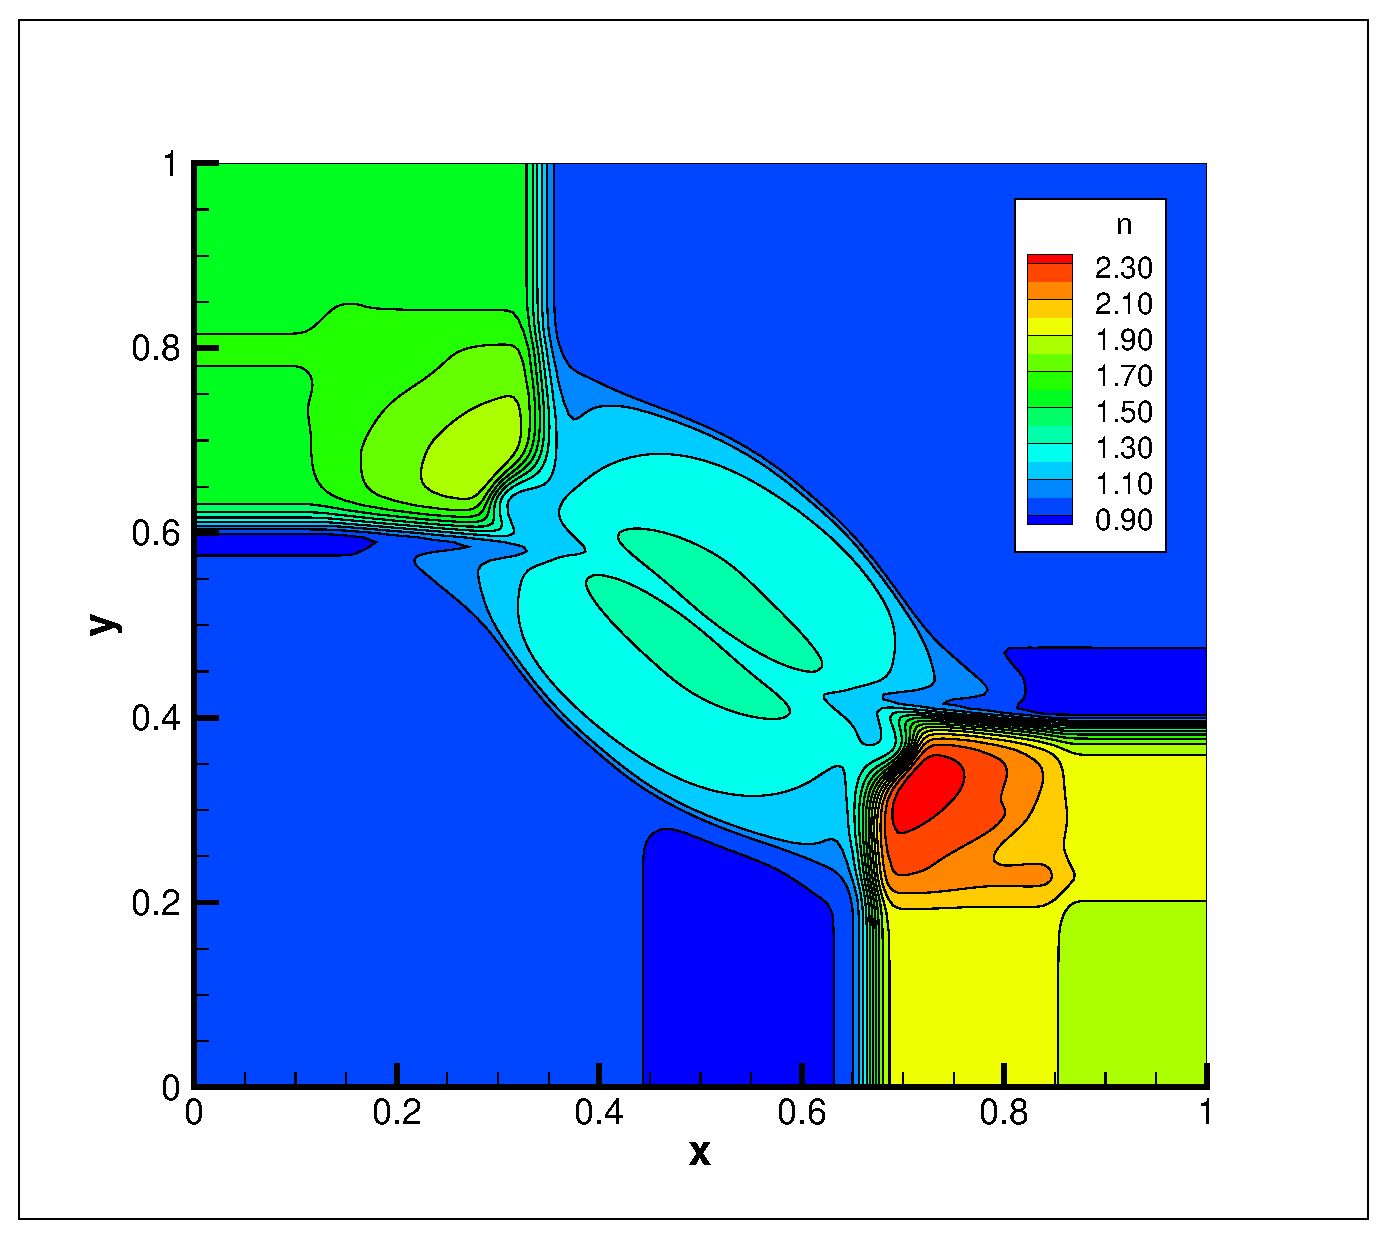
\includegraphics[trim = 20mm 15mm 20mm 20mm,clip,width=\textwidth]{ESBGK_MB_n}
                \caption{Density contour, \\ \it{MB statistic}}
                \label{fig:5ESBGK_MB_n}
        \end{subfigure}
        ~ %add desired spacing between images, e. g. ~, \quad, \qquad etc.
          %(or a blank line to force the subfigure onto a new line)
        \begin{subfigure}[b]{0.32\textwidth}
                \centering
                \includegraphics[trim = 20mm 15mm 20mm 20mm,clip,width=\textwidth]{ESBGK_MB_p}
                \caption{Pressure contour, \\ \it{MB statistic}}
                \label{fig:5ESBGK_MB_p}
        \end{subfigure}
				~ %add desired spacing between images, e. g. ~, \quad, \qquad etc.
          %(or a blank line to force the subfigure onto a new line)
        \begin{subfigure}[b]{0.32\textwidth}
                \centering
                \includegraphics[trim = 20mm 15mm 20mm 20mm,clip,width=\textwidth]{ESBGK_MB_z}
                \caption{Fugacity contour, \\ \it{MB statistic}}
                \label{fig:5ESBGK_MB_z}
        \end{subfigure}
        ~ %add desired spacing between images, e. g. ~, \quad, \qquad etc.
          %(or a blank line to force the subfigure onto a new line)
        \begin{subfigure}[b]{0.32\textwidth}
                \centering
                \includegraphics[trim = 20mm 15mm 20mm 20mm,clip,width=\textwidth]{ESBGK_FD_n}
                \caption{Density contour, \\ \it{FD statistic}}
                \label{fig:5ESBGK_FD_n}
        \end{subfigure}
        ~ %add desired spacing between images, e. g. ~, \quad, \qquad etc.
          %(or a blank line to force the subfigure onto a new line)
        \begin{subfigure}[b]{0.32\textwidth}
                \centering
                \includegraphics[trim = 20mm 15mm 20mm 20mm,clip,width=\textwidth]{ESBGK_FD_p}
                \caption{Pressure contour, \\ \it{FD statistic}}
                \label{fig:5ESBGK_FD_p}
        \end{subfigure}
				~ %add desired spacing between images, e. g. ~, \quad, \qquad etc.
          %(or a blank line to force the subfigure onto a new line)
        \begin{subfigure}[b]{0.32\textwidth}
                \centering
                \includegraphics[trim = 20mm 15mm 20mm 20mm,clip,width=\textwidth]{ESBGK_FD_z}
                \caption{Fugacity contour, \\ \it{FD statistic}}
                \label{fig:5ESBGK_FD_z}
        \end{subfigure}
				\caption{Test on configuration 5 using ES equilibrium distribution function with dimensionless parameter $b=0.5$ and TVD spatial discretization method} \label{fig:test_configuration5}
\end{figure}

\begin{figure}
        \centering
        \begin{subfigure}[b]{0.32\textwidth}
                \centering
                \includegraphics[trim = 20mm 15mm 20mm 20mm,clip,width=\textwidth]{17ESBGK_BE_n}
                \caption{Density contour using BE statistic}
                \label{fig:17ESBGK_BE_n}
        \end{subfigure}%
        ~ %add desired spacing between images, e. g. ~, \quad, \qquad etc.
          %(or a blank line to force the subfigure onto a new line)
        \begin{subfigure}[b]{0.32\textwidth}
                \centering
                \includegraphics[trim = 20mm 15mm 20mm 20mm,clip,width=\textwidth]{17ESBGK_BE_p}
                \caption{Pressure contour using BE statistic}
                \label{fig:17ESBGK_BE_p}
        \end{subfigure}
        ~ %add desired spacing between images, e. g. ~, \quad, \qquad etc.
          %(or a blank line to force the subfigure onto a new line)
        \begin{subfigure}[b]{0.32\textwidth}
                \centering
                \includegraphics[trim = 20mm 15mm 20mm 20mm,clip,width=\textwidth]{17ESBGK_BE_z}
                \caption{Fugacity contour using BE statistic}
                \label{fig:17ESBGK_BE_z}
        \end{subfigure}
				~ %add desired spacing between images, e. g. ~, \quad, \qquad etc.
          %(or a blank line to force the subfigure onto a new line)
        \begin{subfigure}[b]{0.32\textwidth}
                \centering
                \includegraphics[trim = 20mm 15mm 20mm 20mm,clip,width=\textwidth]{17ESBGK_MB_n}
                \caption{Density contour using MB statistic}
                \label{fig:17ESBGK_MB_n}
        \end{subfigure}
        ~ %add desired spacing between images, e. g. ~, \quad, \qquad etc.
          %(or a blank line to force the subfigure onto a new line)
        \begin{subfigure}[b]{0.32\textwidth}
                \centering
                \includegraphics[trim = 20mm 15mm 20mm 20mm,clip,width=\textwidth]{17ESBGK_MB_p}
                \caption{Pressure contour using MB statistic}
                \label{fig:17ESBGK_MB_p}
        \end{subfigure}
				~ %add desired spacing between images, e. g. ~, \quad, \qquad etc.
          %(or a blank line to force the subfigure onto a new line)
        \begin{subfigure}[b]{0.32\textwidth}
                \centering
                \includegraphics[trim = 20mm 15mm 20mm 20mm,clip,width=\textwidth]{17ESBGK_MB_z}
                \caption{Fugacity contour using MB statistic}
                \label{fig:17ESBGK_MB_z}
        \end{subfigure}
        ~ %add desired spacing between images, e. g. ~, \quad, \qquad etc.
          %(or a blank line to force the subfigure onto a new line)
        \begin{subfigure}[b]{0.32\textwidth}
                \centering
                \includegraphics[trim = 20mm 15mm 20mm 20mm,clip,width=\textwidth]{17ESBGK_FD_n}
                \caption{Density contour using FD statistic}
                \label{fig:17ESBGK_FD_n}
        \end{subfigure}
        ~ %add desired spacing between images, e. g. ~, \quad, \qquad etc.
          %(or a blank line to force the subfigure onto a new line)
        \begin{subfigure}[b]{0.32\textwidth}
                \centering
                \includegraphics[trim = 20mm 15mm 20mm 20mm,clip,width=\textwidth]{17ESBGK_FD_p}
                \caption{Pressure contour using FD statistic}
                \label{fig:17ESBGK_FD_p}
        \end{subfigure}
				~ %add desired spacing between images, e. g. ~, \quad, \qquad etc.
          %(or a blank line to force the subfigure onto a new line)
        \begin{subfigure}[b]{0.32\textwidth}
                \centering
                \includegraphics[trim = 20mm 15mm 20mm 20mm,clip,width=\textwidth]{17ESBGK_FD_z}
                \caption{Fugacity contour using FD statistic}
                \label{fig:17ESBGK_FD_z}
        \end{subfigure}
				\caption{Test on configuration 17 using ES equilibrium distribution function with dimensionless parameter $b=0.5$ and TVD spatial discretization method} \label{fig:test_configuration17}
\end{figure}


In this configuration, shock, slip discontinuity and rarefaction fan are expected to be seen propagating from interfaces of the four quadrants. A shock shall be seen propagating through quadrants 3 and 2, rarefaction fan through quadrants 4 and 1 and slip discontinuities through quadrants 2 and 1 and through quadrants 4 and 1.

In Figs. \ref{differenttau} and \ref{differenttaub}  we can see the density plot of Configuration 5 and 17 respectively for Bose-Einstein,  Maxwell-Boltzmann and Fermi-Diract gases with the application of $\tau=0.0005$ and $\tau=0.01$. In these figures, we see more of the effect of dissipation as the value of $\tau$ increases. For example, at $\tau=0.01$ we can see how the flow profiles become very smeared compared to the results with smaller relaxation time values.

\subsection{Comparison of Kinetic Equilibrium Distribution Functions}
Here we test our Algorithm using three statistics using ES and traditional Equilibrium distribution functions.

\begin{figure}
        \centering
        \begin{subfigure}[b]{0.32\textwidth}
                \centering
                \includegraphics[trim = 20mm 15mm 20mm 20mm,clip,width=\textwidth]{ESBGK_BE_n}
                \caption{Fugacity contour using BE statistic and \it{b=0.5}. (Conf. 5)}
                \label{fig:ESBGK_BE_n}
        \end{subfigure}%
        ~ %add desired spacing between images, e. g. ~, \quad, \qquad etc.
          %(or a blank line to force the subfigure onto a new line)
        \begin{subfigure}[b]{0.32\textwidth}
                \centering
                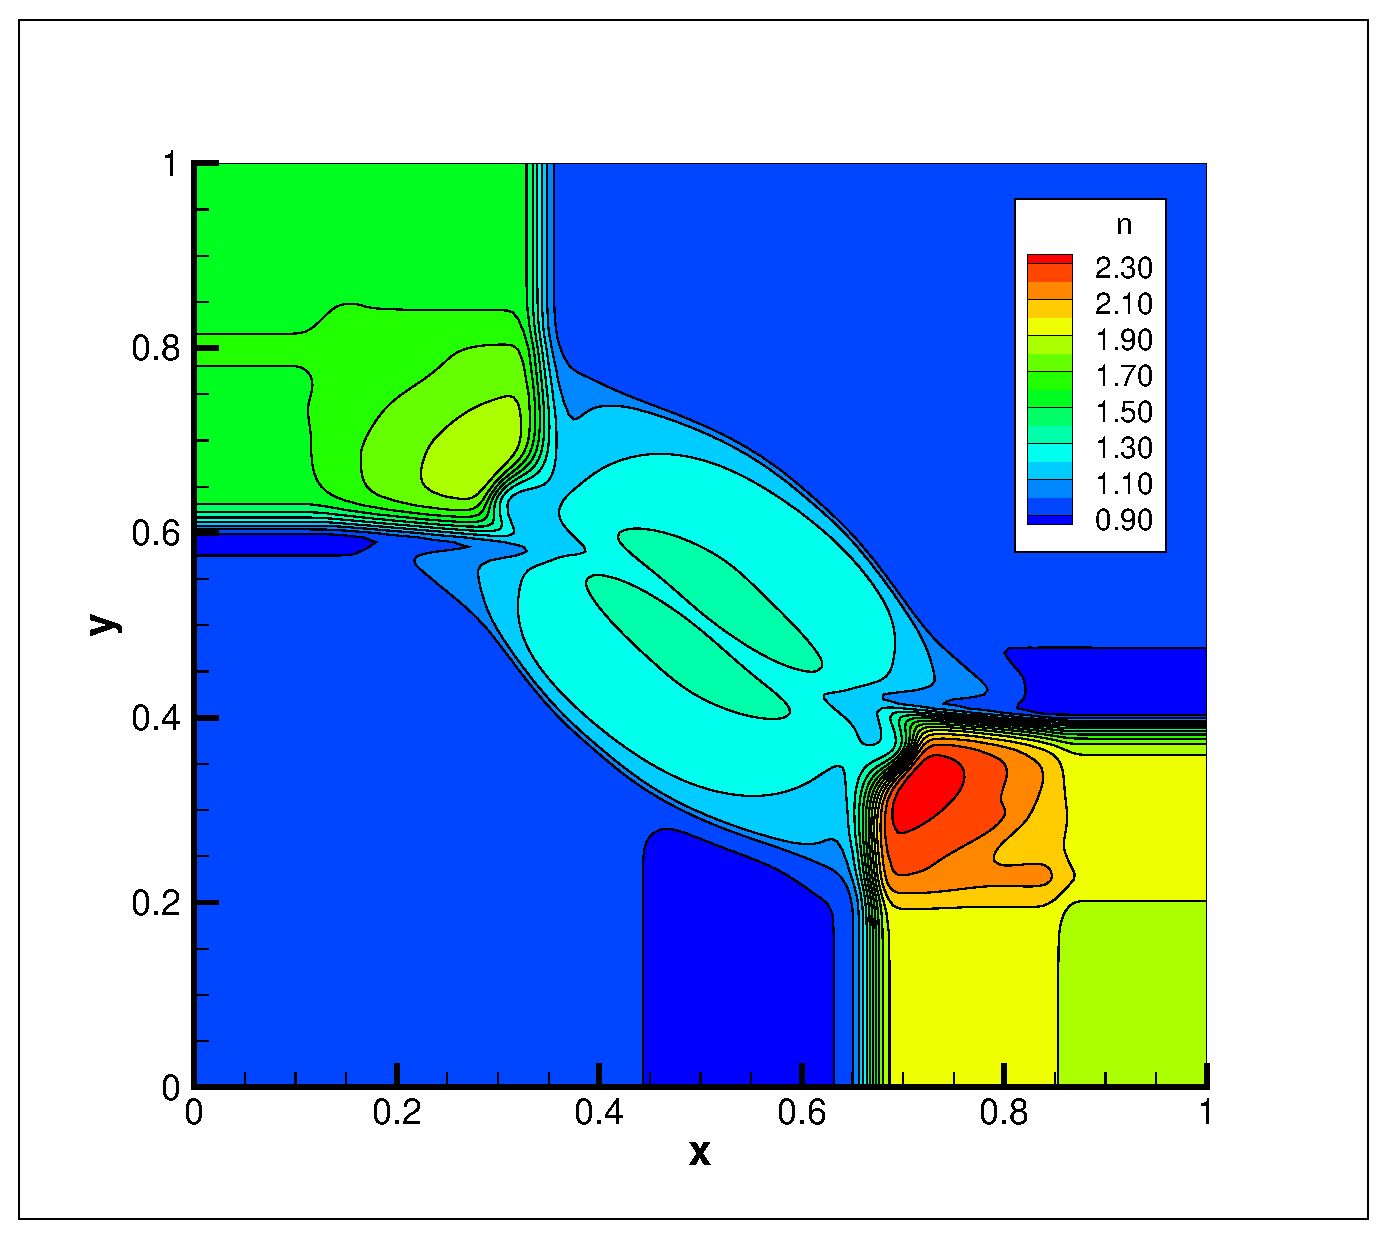
\includegraphics[trim = 20mm 15mm 20mm 20mm,clip,width=\textwidth]{ESBGK_MB_n}
                \caption{Fugacity contour using MB statistic and \it{b=0.5}. (Conf. 5)}
                \label{fig:ESBGK_MB_n}
        \end{subfigure}
        ~ %add desired spacing between images, e. g. ~, \quad, \qquad etc.
          %(or a blank line to force the subfigure onto a new line)
        \begin{subfigure}[b]{0.32\textwidth}
                \centering
                \includegraphics[trim = 20mm 15mm 20mm 20mm,clip,width=\textwidth]{ESBGK_FD_n}
                \caption{Fugacity contour using FD statistic and \it{b=0.5}. (Conf. 5)}
                \label{fig:ESBGK_FD_n}
        \end{subfigure}
        ~ %add desired spacing between images, e. g. ~, \quad, \qquad etc.
          %(or a blank line to force the subfigure onto a new line)
        \begin{subfigure}[b]{0.32\textwidth}
                \centering
                \includegraphics[trim = 20mm 15mm 20mm 20mm,clip,width=\textwidth]{BGK_BE_n}
                \caption{Fugacity contour using BE statistic and \it{b=0}. (Conf. 5)}
                \label{fig:BGK_BE_n}
        \end{subfigure}%
        ~ %add desired spacing between images, e. g. ~, \quad, \qquad etc.
          %(or a blank line to force the subfigure onto a new line)
        \begin{subfigure}[b]{0.32\textwidth}
                \centering
                \includegraphics[trim = 20mm 15mm 20mm 20mm,clip,width=\textwidth]{BGK_MB_n}
                \caption{Fugacity contour using MB statistic and \it{b=0}. (Conf. 5)}
                \label{fig:BGK_MB_n}
        \end{subfigure}
        ~ %add desired spacing between images, e. g. ~, \quad, \qquad etc.
          %(or a blank line to force the subfigure onto a new line)
        \begin{subfigure}[b]{0.32\textwidth}
                \centering
                \includegraphics[trim = 20mm 15mm 20mm 20mm,clip,width=\textwidth]{BGK_FD_n}
                \caption{Fugacity contour using FD statistic and \it{b=0}. (Conf. 5)}
                \label{fig:BGK_FD_n}
        \end{subfigure}
        \caption{Comparison of kinetic results between traditional and ES equilibrium distribution functions}\label{fig:compare_feq}
\end{figure}

\subsection{Comparison of Prant Numbers}
In this subsection, we present the result using refined grid mesh of $200 \times 200$ points using (i) WENO3 scheme and (ii) TVD scheme for the purpose of comparison. Here, the usage of TVD scheme instead of WENO3 scheme is the only difference between the two cases, while other initial attributes are applied similarly. Note that all the previous two dimensional examples shown are generated using $200 \times 200$ grid points. Thus this example also gives us illustration of high mesh points convergence. The problem is initially set for Bose gas with $\tau = 0.0001$. The initial condition of Bose gas is set following Eq. \ref{init5} (Config. 5). The CFL numbers are set to be 0.1. The quadrature rule used is Gauss-Hermite rule with 20 abscissas both in $\upsilon_x$ and $\upsilon_y$ directions.

\begin{figure}
        \centering
        \begin{subfigure}[b]{0.32\textwidth}
                \centering
                \includegraphics[trim = 20mm 15mm 20mm 20mm,clip,width=\textwidth]{ESBGK_FD_bn05_n}
                \caption{Density contour using MB statistic and ES model with $\it{b=-0.5}$.}
                \label{fig:ESBGK_FD_bn05_n}
        \end{subfigure}%
        ~ %add desired spacing between images, e. g. ~, \quad, \qquad etc.
          %(or a blank line to force the subfigure onto a new line)
        \begin{subfigure}[b]{0.32\textwidth}
                \centering
                \includegraphics[trim = 20mm 15mm 20mm 20mm,clip,width=\textwidth]{BGK_FD_b0_n}
                \caption{Density contour using MB statistic and ES model with $\it{b=0}$.}
                \label{fig:BGK_FD_b0_n}
        \end{subfigure}
        ~ %add desired spacing between images, e. g. ~, \quad, \qquad etc.
          %(or a blank line to force the subfigure onto a new line)
        \begin{subfigure}[b]{0.32\textwidth}
                \centering
                \includegraphics[trim = 20mm 15mm 20mm 20mm,clip,width=\textwidth]{ESBGK_FD_bp05_n}
                \caption{Density contour using MB statistic and ES model with $\it{b=0.5}$.}
                \label{fig:ESBGK_FD_bp05_n}
        \end{subfigure}
        \caption{Using Configuration 5 to test kinetic influence of dimensionales parameter \it{b}.}\label{fig:test_b_parameter}
\end{figure}

\subsection{Observations of the pressure tensor components}

\begin{figure}
        \centering
        \begin{subfigure}[b]{0.32\textwidth}
                \centering
                \includegraphics[trim = 20mm 15mm 20mm 20mm,clip,width=\textwidth]{ESBGK_MB_pxx}
                \caption{$P_{xx}$ contour using MB statistic and $\it{b=0.5}$.}
                \label{fig:5ESBGK_MB_pxx}
        \end{subfigure}%
        ~ %add desired spacing between images, e. g. ~, \quad, \qquad etc.
          %(or a blank line to force the subfigure onto a new line)
        \begin{subfigure}[b]{0.32\textwidth}
                \centering
                \includegraphics[trim = 20mm 15mm 20mm 20mm,clip,width=\textwidth]{ESBGK_MB_pxy}
                \caption{$P_{xy}$ contour using MB statistic and $\it{b=0.5}$.}
                \label{fig:5ESBGK_MB_pxy}
        \end{subfigure}
        ~ %add desired spacing between images, e. g. ~, \quad, \qquad etc.
          %(or a blank line to force the subfigure onto a new line)
        \begin{subfigure}[b]{0.32\textwidth}
                \centering
                \includegraphics[trim = 20mm 15mm 20mm 20mm,clip,width=\textwidth]{ESBGK_MB_pyy}
                \caption{$P_{yy}$ contour using MB statistic and $\it{b=0.5}$.}
                \label{fig:5ESBGK_MB_pyy}
        \end{subfigure}
        \caption{Pressure Tensor components of configuration 5}\label{fig:conf5_pTensor}
\end{figure}

\begin{figure}
        \centering
        \begin{subfigure}[b]{0.32\textwidth}
                \centering
                \includegraphics[trim = 20mm 15mm 20mm 20mm,clip,width=\textwidth]{17ESBGK_FD_pxx}
                \caption{$P_{xx}$ contour using FD statistic and $\it{b=0.5}$.}
                \label{fig:17ESBGK_FD_pxx}
        \end{subfigure}%
        ~ %add desired spacing between images, e. g. ~, \quad, \qquad etc.
          %(or a blank line to force the subfigure onto a new line)
        \begin{subfigure}[b]{0.32\textwidth}
                \centering
                \includegraphics[trim = 20mm 15mm 20mm 20mm,clip,width=\textwidth]{17ESBGK_FD_pxy}
                \caption{$P_{xy}$ contour using FD statistic and $\it{b=0.5}$.}
                \label{fig:17ESBGK_FD_pxy}
        \end{subfigure}
        ~ %add desired spacing between images, e. g. ~, \quad, \qquad etc.
          %(or a blank line to force the subfigure onto a new line)
        \begin{subfigure}[b]{0.32\textwidth}
                \centering
                \includegraphics[trim = 20mm 15mm 20mm 20mm,clip,width=\textwidth]{17ESBGK_FD_pyy}
                \caption{$P_{yy}$ contour using FD statistic and $\it{b=0.5}$.}
                \label{fig:17ESBGK_FD_pyy}
        \end{subfigure}
        \caption{Pressure Tensor components of configuration 17}\label{fig:conf5_pTensor}
\end{figure}


In Fig. \ref{WENOTVD2D}, we can see the comparison in which WENO3 outperform TVD in terms of flow profiles sharpness when set within the same numerical treatment. Although the kind of gas used in this example is Bose gas, the results are comparable to the earlier work of Lax \cite{Laxliu95} (classical gas) in terms of the expected form of flows. Note that the application of constant relaxation time, although small, contribute to a more diffusive form of flows.

\section{Concluding Remarks}
\label{remarks}
The new semiclassical ellipsoidal statistical equilibrium distribution of Wu et al. \cite{Wu2012} has been derived through maximum entropy principle and conserves the mass, momentum and energy but differs from the standard Bose-Einstein or Fermi-Dirac distribution.  This ES distribution is anisotropic thus it can possess additional high order moments, thus its gas dynamical features are not well known and are worth exploring.   In this work, the unsteady quantum gas dynamical flow features as dictated by the semiclassical ellipsoidal statistical equilibrium distribution function is numerically studied.   The computational method treats the governing equation in phase space and employs the discrete ordinate method and high resolution shock capturing schemes.  Specifically, we describe the solution method in details for the equation in two space dimensions.   The present decoding method for the semiclassical ellipsoidal statistical distribution is different from the that for Bose-Einstein or Fermi-Dirac distribution.   Computations of two-dimensional Riemann problems for gas flows of arbitrary particle statistics are presented.  These computational examples serve the purpose of exploring the nonlinear manifestation of shock wave, contact line and rarefaction wave and testing the robustness of the present method.   All the expected flow profiles comprising shock, rarefaction wave and contact discontinuities and their nonlinear interactions can be observed with considerably good detail and are in consistency with available results.   The present work emphasizes on building the unified and parallel framework for treating semiclassical gas dynamics.   Direct extension to three-dimensional cases and more complex geometries in general coordinates are straightforward and will be reported elsewhere.

%%Hsieh & Yang (2009) T. Y. Hsieh and J. Y. Yang, Thermal conductivity modeling of nanowire composites, J. Applied Physics, 108, 023528 (2010).

\section{Acknowledgements*}
\label{Acknowledgements}
The authors thank Dr. J. C. Huang and Dr. Y. H. Shi for many fruitful discussions. The authors also like to acknowledge the National
Center for High-Performance Computing in providing resources
under the national project gKnowledge Innovation National Gridh in Taiwan.

This work is done under the auspices of National Science Council, TAIWAN through grants NSC-99-2922-I-606-002 and CQSE subproject No. 5 99R-80873.
%%%%%%%%%% Insert bibliography here %%%%%%%%%%%%%%

%\begin{thebibliography}{9}

%\bibitem{1} Allwood JM, Cullen JM. 2011 \textit{Sustainable materials:  with both eyes open}.
%Cambridge, UK: UIT Cambridge. See \href{http://www.withbotheyesopen.com}{http://www.withbotheyesopen.com}.

%\bibitem{2}  MacKay DJC. 2008  \textit{Sustainable energy:  without the hot air}.
% Cambridge, UK: UIT Cambridge. See \href{http://www.withouthotair.com}{http://www.withouthotair.com}.

%\bibitem{3} Gallman PG. 2011  \textit{Green alternatives and national energy strategy: the facts
% behind the headlines}.  Baltimore,\ MD: Johns Hopkins University Press.

%\bibitem{4} MacKay DJC. 2013.  Solar energy in the context of energy use, energy transportation, and
% energy storage. \textit{Proc. R. Soc. A} \textbf{371}.

%\end{thebibliography}

\bibliographystyle{siam}
\bibliography{SB-ESBGK}

\end{document}
